

\begin{figure*}[!htb]
\begin{minipage}[c]{0.33\textwidth}
  \centering
  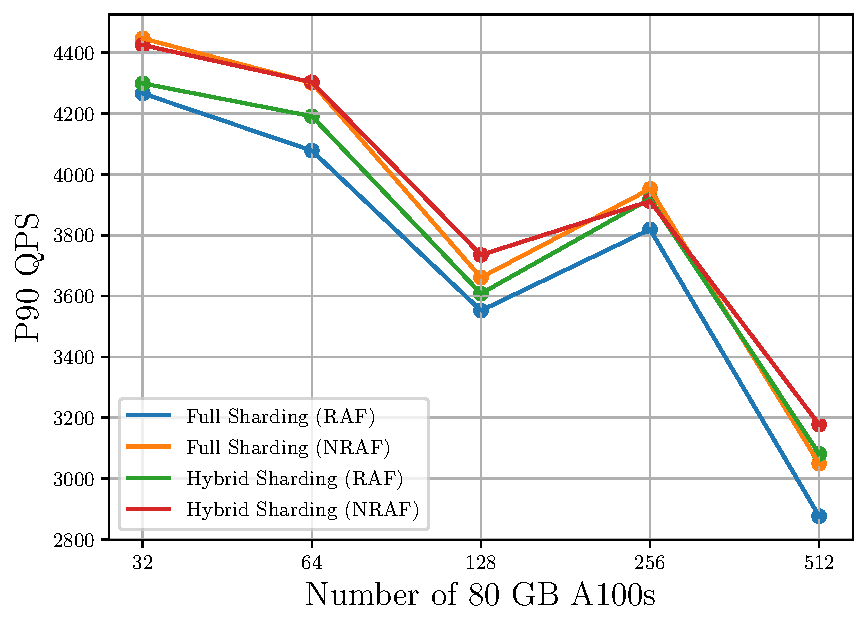
\includegraphics[width=\linewidth]{figure/dhen_qps.pdf}
  (a) DHEN QPS
\end{minipage}
\begin{minipage}[c]{0.33\textwidth}
  \centering
  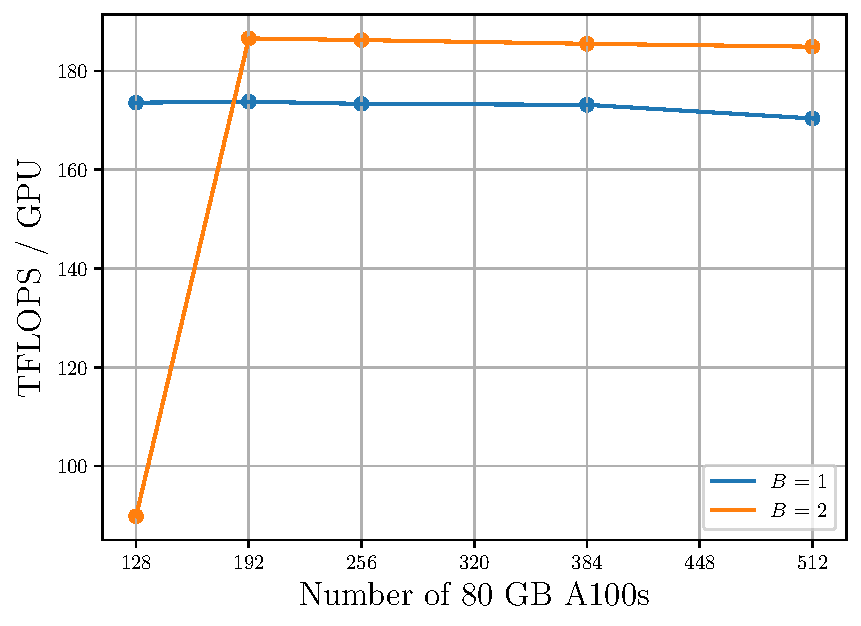
\includegraphics[width=\linewidth]{figure/tflops_scaling_175b.pdf}
  (b) GPT-175B TFLOPS
\end{minipage}
\begin{minipage}[c]{0.33\textwidth}
  \centering
  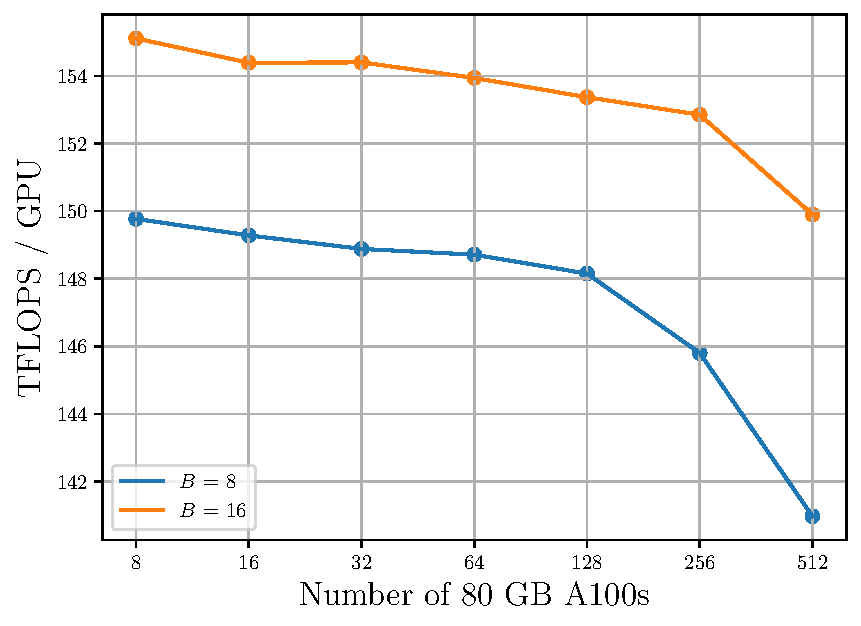
\includegraphics[width=\linewidth]{figure/tflops_scaling_t5.pdf}
  (c) T5-11B TFLOPS
\end{minipage}
%\vspace{-1em}
\caption{Training Throughput: To conform with DHEN convention, we use sample/ GPU/second (QPS) for DHEN.}\label{fig:throughput}
%\vspace{-1em}
\end{figure*}



\begin{figure*}[!htb]
\begin{minipage}[c]{0.33\textwidth}
  \centering
  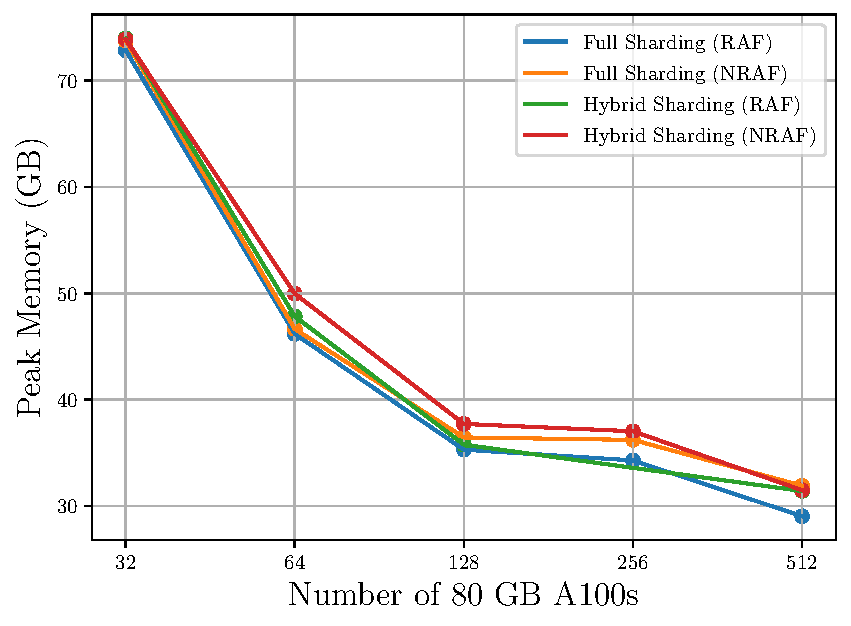
\includegraphics[width=\linewidth]{figure/dhen_mem.pdf}
  (a) DHEN
\end{minipage}
\begin{minipage}[c]{0.33\textwidth}
  \centering
  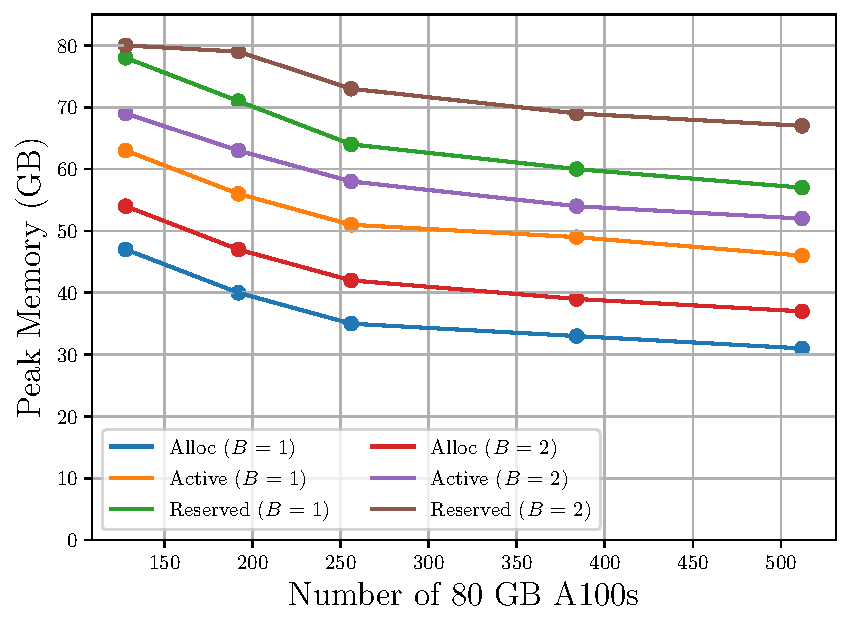
\includegraphics[width=\linewidth]{figure/mem_scaling_175b.pdf}
  (b) GPT-175B
\end{minipage}
\begin{minipage}[c]{0.33\textwidth}
  \centering
  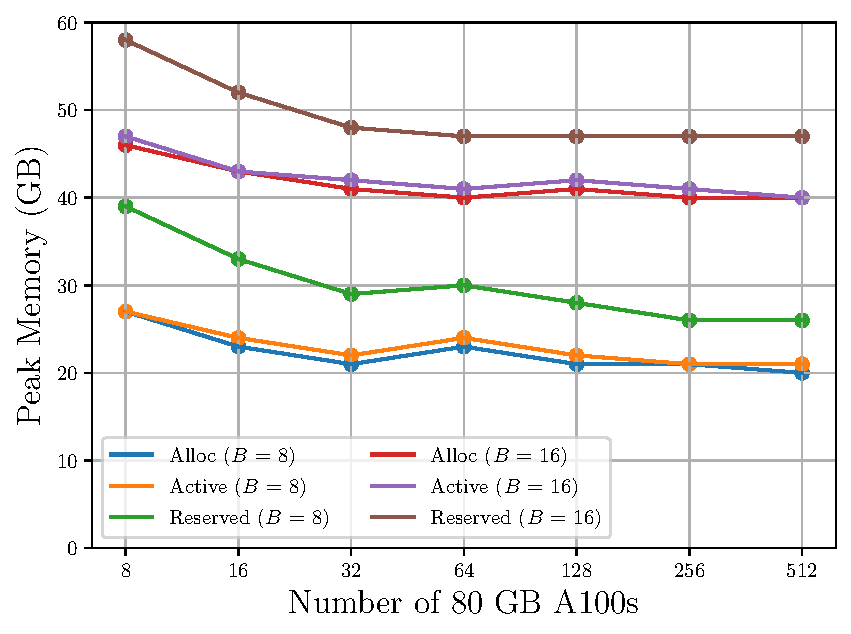
\includegraphics[width=\linewidth]{figure/mem_scaling_t5.pdf}
  (c) T5-11B
\end{minipage}
%\vspace{-1em}
\caption{Memory Footprint}\label{fig:memory}
%\vspace{-1em}
\end{figure*}

\subsection{Efficient Training for Large Models}\label{sec:eval_prod}

To evaluate capability of using FSDP for large models, we ran three types of models using Full Sharding with prefetching and rate limiter turned on. Activation checkpointing and \code{BF16} mixed precision are also applied in these experiments. Adam optimizer is used to reflect a production workload setup and to incur the costly two optimizer states per parameter.
\begin{itemize}
    \item \textbf{DHEN large recommendation model}~\cite{DHEN}: model size - 768B sparse parameters and 550M dense parameters, and batch size 1024. 
    \item \textbf{minGPT transformer}~\cite{MinGPT}: model size 175B, vocab size 50000, block size 2048, batch size 1 and 2 for 128, 192, 256, 384 and 512 GPUs.
    \item \textbf{HuggingFace T5 transformer}~\cite{raffel2020exploring}: model size 11B, sequence length 512, batch size 8 and 16 for 8, 16, 32, 64, 128, 256, 512 GPUs.
\end{itemize}

In the DHEN experiments, we further combine sharding strategies with two different configurations: 

\begin{itemize}
    \item \textbf{RAF:} reshard-after-forward frees \code{AllGather}ed shards from other GPUs after forward pass and unshards them again before backward computation. This reduces peak memory consumption at the cost of higher communication overhead.
    \item \textbf{NRAF:} no-reshard-after-forward is the opposite where the unsharded model parameters stay in GPU memory after forward pass until backward computations finish, which trades higher memory footprint for lower communication overhead.
\end{itemize}

The experimental results in Figure~\ref{fig:throughput}~(a) and Figure~\ref{fig:memory}~(a) indicate that FSDP is capable of accommodating DHEN models on a large GPU cluster. It was observed that Full Sharding with RAF yields the smallest memory footprint but with a corresponding trade-off of reduced QPS. Conversely, Hybrid Sharding with NRAF demonstrated the opposite behavior, as it has employs both a smaller sharding group and skips one reshard. When adding more GPUs to in the cluster, the peak memory usage consistently decreases as a result of a decrease in the size of each rank's model shard.

With the 175B model, the experiments achieved more than 173 and 186 TFLOPS per GPU with batch size equal to 1 and 2 respectively as shown in Figure~\ref{fig:throughput}~(b). This is equivalent to approximately 55\% and 60\% of GPU hardware utilization, given that the A100's peak is 312 TFLOPS using the \code{BF16} tensor core. Furthermore, the model demonstrated linear scalability from 128 GPUs to 512 GPUs, in terms of TFLOPS, which affirms the efficacy of FSDP in handling large models with expensive computations or high-speed network interconnections. Notably, with 128 GPUs, setting the batch size to 2 resulted in a considerably lower per-GPU TFLOPs in comparison to other scenarios. This was due to CUDA memory defragmentation during the backward pass. The backward pass contributed 85.56\% of the iteration latency for the 128 GPU batch size equals 2 case, while a normal backward pass only accounted for about 67\% in these experiments. Using 128 GPUs is more likely to trigger defragmentation, as each GPU needs to accommodate a larger model shard. Figure~\ref{fig:memory} confirms this explanation, where the PyTorch CUDA caching allocator depletes all 80GB of the CUDA memory as shown on the top left corner. 


Finally, for T5-11B models as shown in Figure~\ref{fig:memory}~(c), all experiments are executed comfortably below GPU memory capacity, where defragmentations are unlikely to happen. Nevertheless, as the number of GPUs increases from 8 to 512, a 7\% regression in per-GPU TFLOPS is still evident as illustrated in Figure~\ref{fig:throughput}~(c). This suggests that communications begin to outweigh computations on large clusters, and a near-perfect overlap between communication and computation is no longer attainable.